\section{Linear Regression}

Implementing linear regression was the first part of the assignment.

\subsection{Introduction}

This assignment was seperated into three parts.
\begin{enumerate}
	\item Data Generation
	\item Implementation of the algorithm
	\item Evaluation of the result
\end{enumerate}

\subsection{Data Generation}
\label{sec:dataGen}

For the linear regression assignment we had specific description about how to generate the dataset. The dataset consists of $51$ points on the quadratic function $2*x^2 + G*x + 1$ where $G$ is the number of our group, which is $5$. For this dataset we also had to generate a trainingdataset, which is $1/6$ in size of the original dataset. Those points are taken from the original dataset and then shifted by a random number chosen by a normal distribution with parameter $\mu = 0$ and $\sigma = 0.6$.

\subsection{Implementation of the algorithm}

In this assignment we used the online learning rule of the gradient descent algorithm. Therefore, every trainingsexample changes the weights. In contrast by using the batch learning technique, we only update after the whole trainingset has been processed. Therefore the weight changes faster with the online learning rule than with the batch learning.

The algorithm works the following way:
\begin{enumerate}
	\item Calculate $\delta$ for the current training example
	\item Update weights according to $\delta$ and $\gamma$.
\end{enumerate}

We are using Sum of Squared Error (SSE) as our cost function and therefore $delta$ can be calculated using $delta = -(y- x't)*x$. Then the weight update is $w(t+1) = w(t) - \gamma*\delta)$.

\subsection{Evaluation of the Results} 

I tested the performance of the gradient descent algorithm on the dataset described in Section \ref{sec:dataGen}. The result can be seen in Figure \ref{fig:perGraDescent}. Additionally I compared it to the result obtained by calculating the optimal weight in Figure \ref{fig:comparision}. As can be seen the weights are nearly identically after converging. 

\begin{figure}[!ht]
		\centering
		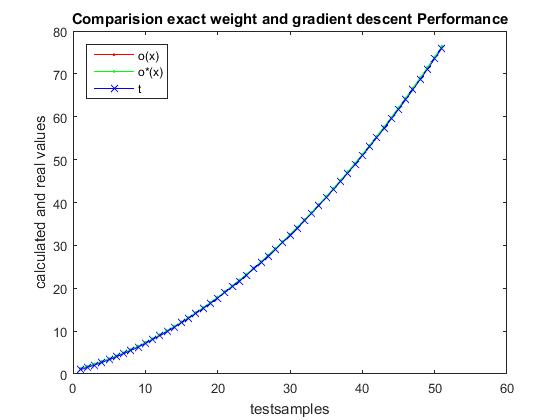
\includegraphics[width=1\textwidth]{img/Comparision}
		\caption{Comparision by gradient descent to the optimal weight}
		\label{fig:comparision}
\end{figure}

\begin{figure}[!ht]
	
	\begin{minipage}{0.5 \textwidth}
		\centering
		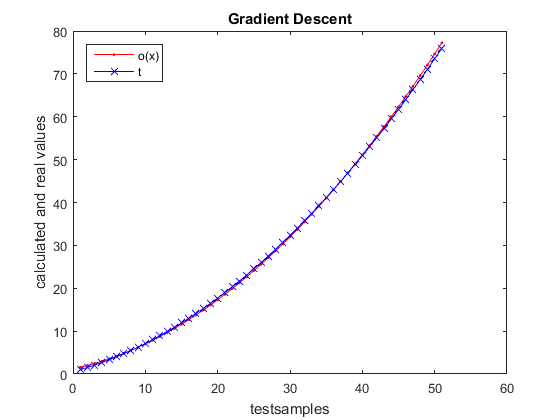
\includegraphics[width=1\textwidth]{img/gradientDescent}
		\caption{Performance by gradient descent on the real dataset}
		\label{fig:perGraDescent}
	\end{minipage}
	\begin{minipage}{0.5 \textwidth}
		\centering
		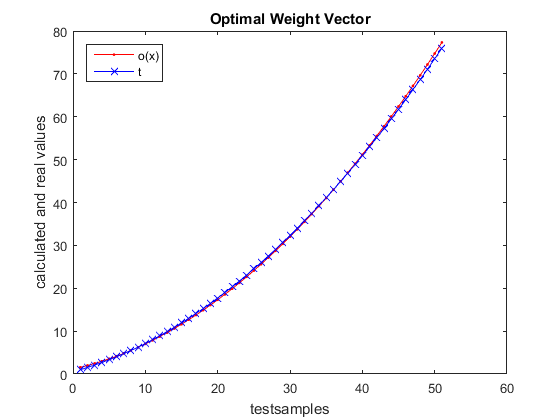
\includegraphics[width=1\textwidth]{img/optimalWeightVector}
		\caption{Performance by the optimal weight on the real dataset}
		\label{fig:perOptimal}
	\end{minipage}
\end{figure}



\subsection{Questions}

\subsubsection{Question 1: What weight vector was calculated using gradient descent?}

We got the weight vector $w = [0.4154, 5.2012, 2.0025]$ for the sample problem after 1000 iterations of gradient descent with the learning rate $\gamma = 0.001$.

\subsubsection{Question 2: How can you calculate the optimal weight directly? How much different is it to the result of gradient descent?}

We can use linear algebra to reformulate the gradient descent problem. After solving the formula we get $w = (XX^T)^{-1}Xt^T$. Therefore, if $XX^T$ is invertible we can use this formula to directly compute the optimal weight vector.

Our test data is randomly generated and the variance to the real data is also at random, therefore the weight vector had small differences in distances to each other. With this procedure we got t the optimal weight vector $w^* = [0.4040, 5.2352, 1.9910]$, whereby the gradient descent weight vector was $w = [0.4154, 5.2012, 2.0025]$. As can be seen in Figure \ref{fig:perGraDescent} and Figure \ref{fig:perOptimal} the result is very similar. This result was obtained with the same testdata, we had used for question 1. 

\subsubsection{Question 3: Which tradeoff exist in choosing $\gamma$ between trainingtime and convergence? Is there a $\gamma$ where gradient descent diverges?}


\begin{figure}[!ht]
	\begin{minipage}{0.5 \textwidth}
		\centering
		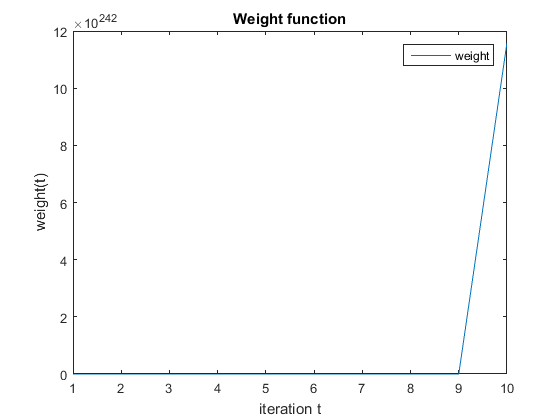
\includegraphics[width=1\textwidth]{img/WeightFunction1}
		\caption{Convergence with $\gamma$ at 1}
		\label{fig:weight1}
	\end{minipage}
	\begin{minipage}{0.5 \textwidth}
		\centering
		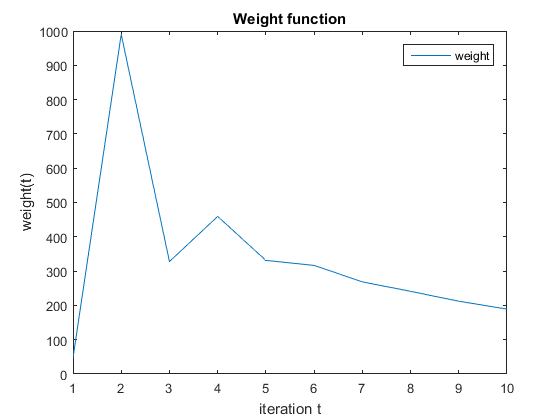
\includegraphics[width=1\textwidth]{img/WeightFunction01}
		\caption{Convergence with $\gamma$ at 0.005}
		\label{fig:weight05}
	\end{minipage}
\end{figure}


\begin{figure}[!ht]
	\begin{minipage}{0.5 \textwidth}
		\centering
		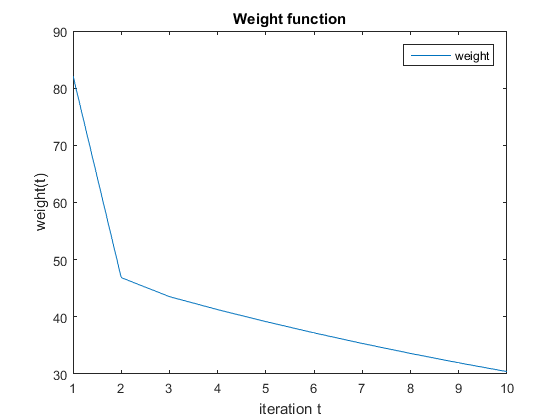
\includegraphics[width=1\textwidth]{img/WeightFunction005}
		\caption{Convergence with $\gamma$ at 0.005}
		\label{fig:weight005}
	\end{minipage}
	\begin{minipage}{0.5 \textwidth}
		\centering
		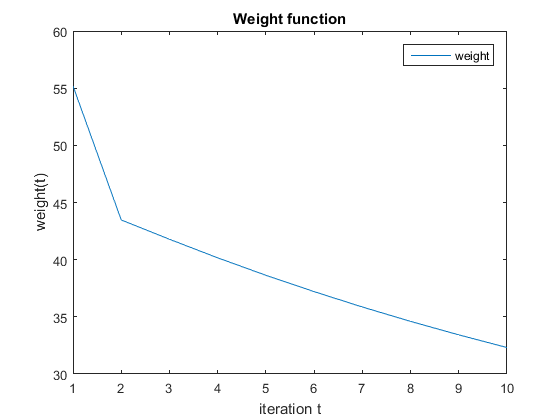
\includegraphics[width=1\textwidth]{img/WeightFunction001}
		\caption{Convergence with $\gamma$ at 0.001}
		\label{fig:weight001}
	\end{minipage}
\end{figure}

As can be seen in Figure \ref{fig:weight1}, \ref{fig:weight1}, \ref{fig:weight05} and \ref{fig:weight001} chosing $\gamma$ is a tradeoff between trainingtime and convergence. Also convergence depends on the random initialization of the training data. However there is a way to make the learning rate smaller in time by setting $\gamma = c/t$, where c is the initial learning rate and t is the current Iteration. For the given training data $\gamma = 1$ diverges as can be seen in Figure \ref{fig:weight1}.





